\item \points{1e}
In \texttt{src/submission.py}, fill in the code to calculate $\phi$, $\mu_{0}$, $\mu_{1}$, and $\Sigma$, use these parameters to derive $\theta$, and use the resulting GDA model to make predictions on the validation set. Make sure to write your model's predictions on the validation set to the file specified in the code.

To verify a correct implementation, run the autograder test case |1e-4-basic| to create a plot of the \textbf{validation data} with $x_1$ on the horizontal axis and $x_2$ on the vertical axis. To visualize the two classes, use a different symbol for examples $x^{(i)}$ with $y^{(i)} = 0$ than for those with $y^{(i)} = 1$. On the same figure, plot the decision boundary found by GDA (i.e, line corresponding to $p(y\vert x) = 0.5$).\\

The output plot should look similar to the following (no plot submission is required): 

\begin{figure}[H]
	\centering
	\vspace{2mm}
	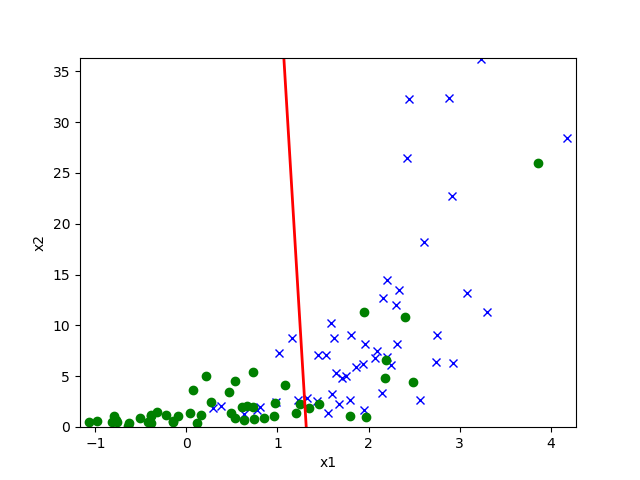
\includegraphics[width=0.65\linewidth]{01-linearclass/p01e_pred_1.png}
    \caption{Separating hyperplane for GDA on the validation set for Dataset 1 (Note: This is for reference only.  You are not required to submit a plot.)}
\end{figure}
